%%%%%%%%% PROPOSAL -- 15 pages (including Prior NSF Support)
% From the NSF Grants Proposal Guide:
% "The Project Description should provide a clear statement of the work 
% to be undertaken and must include: objectives for the period of the proposed 
% work and expected significance; relation to longer-term goals of the PI's 
% project; and relation to the present state of knowledge in the field, 
% to work in progress by the PI under other support and to work in progress 
% elsewhere."

%\required{Project Description}
\section{Project Description}

\subsection{Agenda}

\subsubsection{Algorithms / Programming}

\begin{figure}[!h]
        \begin{center}
		%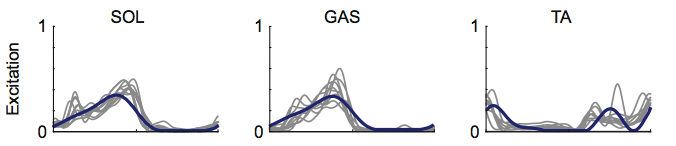
\includegraphics[width=120mm]{images/excite}
                \caption{Some great figure}
                \label{curves}
        \end{center}
\end{figure}


\subsection{Methodology}
%this section should talk about how the team will develop, maybe software
% processes, and how to get customer feedback

\subsubsection{Project Software}
TODO: This project will be written in Ruby on Rails or some other great 
MVC, will install on Windows, Linux, and Mac, blah blah blah. It will be 
downloadable to customers via a private github, Apple's App Store,
or some other overpriced method. Consulting to set it up won't exist because
the whole thing installs itself, and everything is so simple. 

\section{Customer}
%Talk about Alex and the Methow, and all the doe they are rolling in to pay
% for this thing.
%Talk about their needs, and the impact this project could have on them.
%Talk also about how future customer, not just in the Basin, but elsewhere
% could benefit from the product.

\section{Statement of Qualifications}
%What gives us the idea we can actually pull this off?

\section{Conclusion}
%Why should people pay for this thing, why should the capstone PM's want
% this project, and why is it great for humanity


%\required{Broader Impacts}
% as in the project summary, broader impacts must be called out separately 
% in the project description.  You may be able to give more specific
% examples, or discuss how you've previously achieved these impacts.
% It should be similar, but not identical, to the Broader Impacts statement
% in the project summary

%\required{Results From Prior NSF Support}
% 5 pages or fewer of the 15 pages for entire description document.
% include results from NSF grants received in the past 5 years.
% if supported by more than one grant, choose the most relevant one
% for each grant, include: NSF award number, amount, dates of
% support, and publications resulting from this research.
% due to space limitations, it is often advisable to use citations rather
% than putting the titles of the publications in the body 
% of this section

% e.g.: "My prior grant, "Uses of Coffee in Mathematical Research" (DMS-0123456, 
% $100,000, 2005-2008), resulted in 3 papers [1],[2],[3], demonstrating..."

% if requesting postdoctoral research salary, a supplemental 1-page document
% called "Postdoc Mentoring Plan" will be required 

